\documentclass[11pt]{article}

\usepackage[margin=1.1in]{geometry}
\usepackage{amsmath,amssymb,amsthm}
\usepackage{booktabs}
\usepackage{microtype}
\usepackage{tikz}
\usetikzlibrary{calc}
\usepackage[colorlinks=true,linkcolor=blue!50!black,urlcolor=blue!50!black]{hyperref}

\newtheorem{theorem}{Theorem}[section]
\newtheorem{lemma}[theorem]{Lemma}
\newtheorem{proposition}[theorem]{Proposition}
\newtheorem{corollary}[theorem]{Corollary}
\theoremstyle{definition}
\newtheorem{definition}[theorem]{Definition}
\newtheorem{remark}[theorem]{Remark}
\newtheorem{construction}[theorem]{Construction}

\newcommand{\lean}[1]{\texttt{#1}}
\newcommand{\file}[1]{\textsf{#1}}
\newcommand{\stepN}{\mathrm{step}}
\newcommand{\Left}{\mathsf{L}}
\newcommand{\Right}{\mathsf{R}}

\title{The State Law for Lazy-Point Train Tracks:\\
  $f(N) = \min(2^N,\, N+4)$}
\author{Carl Heise\thanks{Human-readable rendering extracted from the
    machine-checked Lean~4 development
    (\texttt{github.com/senegrom/duplotrain}, directory
    \file{theory/lean}); prepared with the assistance of Claude (Anthropic).
    The formal proof is the authority: every numbered statement below is a
    theorem of that development, and the sharp upper bound
    (Section~\ref{sec:upper}) is presented as a faithful account of the
    formal argument rather than an independent proof.}}
\date{August 2026}

\begin{document}
\maketitle

\begin{abstract}
  A single train drives forever over a layout of $N$ three-way switches
  with \emph{lazy points}: entering at the stem, the train follows the
  current tongue and moves nothing; entering at a branch, it forces the
  tongue to that branch and leaves by the stem.  How many distinct
  settings of the $N$ tongues can one train ever exhibit?  Exactly
  \[ f(N) \;=\; \min\bigl(2^N,\; N+4\bigr) \qquad\text{for every } N \ge 0. \]
  The bound is uniform over all layouts, all starting positions, and all
  initial tongue settings; it is attained, for every $N$, by an explicit
  layout.  The whole law is machine-checked as a single Lean~4 theorem,
  \lean{GeneralN.state\_law}, built without Mathlib, whose axiom audit is
  exactly the three standard Lean axioms.  This document is a
  human-readable rendering of that proof: complete for the model, the
  $2^N$ ceiling, and every attainment construction, and a structured
  account of the sharp $N+4$ upper bound.
\end{abstract}

\tableofcontents

\section{Introduction}

The question comes from a toy: LEGO\textsuperscript{\textregistered}
DUPLO\textsuperscript{\textregistered} train track.  Its Y-switches have
unsprung, \emph{lazy} points.  A train entering the switch at its single
stem is routed by whatever position the tongue happens to be in, and the
tongue does not move.  A train entering through one of the two branches
pushes the points aside if necessary --- the tongue ends up aimed at the
branch the train came in by --- and exits through the stem.  A layout wires
the free ends of switches to one another with plain track; plain track has
no state, so the machine state of a layout is the vector of its $N$ tongue
positions, one bit per switch.

A single train, placed anywhere, either eventually falls off an unwired
end or drives forever.  Along the way the tongue vector changes.  The
\emph{state count} of a run is the number of distinct tongue vectors it
exhibits; $f(N)$ is the maximum state count over all $N$-switch layouts,
all starts, and all initial tongue vectors.  Trivially $f(N) \le 2^N$.
The surprise is how far below $2^N$ the truth lies:

\begin{theorem}[The state law]\label{thm:main}
  For every $N \ge 0$,
  \[ f(N) \;=\; \min\bigl(2^N,\; N+4\bigr). \]
  That is: no run on any $N$-switch layout ever exhibits more than
  $\min(2^N, N+4)$ distinct tongue vectors, and for every $N$ some layout,
  start, and initial setting exhibits exactly that many.
\end{theorem}

One train can barely move the machine it drives over: of the $2^N$
conceivable switch settings, all but $N+4$ are unreachable within any
single run, no matter how the track is laid.  The $2^N$ leg of the
minimum binds only for $N \le 2$ ($f(0)=1$, $f(1)=2$, $f(2)=4$); from
three switches on, $f(N) = N+4$.

The result was found and proved formally.  A sequence of machine-checked
bounds
\[ 26N{+}3 \to 24N{+}5 \to 18N{+}3 \to \cdots \to 2N{+}9 \to N{+}7 \to
   N{+}6 \to N{+}5 \to N{+}4 \]
was tightened until the constructive lower bound was met.  The final
development (about $28{,}500$ lines of Lean~4 in $70$ files, using no
external mathematics library) proves the single statement
\begin{center}
  \lean{GeneralN.state\_law :\ }$\forall N$,
  \lean{IsExactStateCount} $N$ $(\min(2^N, N+4))$
\end{center}
and audits it to exactly the axioms
$\{\lean{propext}, \lean{Classical.choice}, \lean{Quot.sound}\}$ ---
in particular with no appeal to native code evaluation: the few finite
computations are checked by the proof kernel itself.

\paragraph{What this document is.}
Sections~\ref{sec:model}--\ref{sec:family} are complete human
mathematics: the model, the ceiling $f(N) \le 2^N$, the resolution of the
minimum, and all attainment constructions, each of which a reader can
verify by hand.  Section~\ref{sec:upper} renders the sharp upper bound
$f(N) \le N+4$ --- by far the deep half, roughly $25{,}000$ formal lines
--- as a structured account: the objects, the main lemmas, and the
charging argument, with enough proof for each step that the shape of the
mathematics is visible, and with pointers into the formal text, which
remains the complete reference.  Section~\ref{sec:formal} records what
was formalised and how to check it.

The physical-trace core of the argument (Section~\ref{ssec:traces})
descends from the first-repeated-track idea in the train-set literature;
the formal sources name Chalcraft--Greene and Aaronson.

\section{The model}\label{sec:model}

Everything is stated over a discrete dynamics in which plain-track
geometry provably never enters; only the wiring pattern matters.

\begin{definition}[Ports and wirings]\label{def:wiring}
  Switch $k$ ($k = 0, 1, 2, \dots$) owns three \emph{ports}, encoded as
  natural numbers: its \emph{stem} $3k$, its \emph{left branch} $3k+1$,
  and its \emph{right branch} $3k+2$.  A \emph{wiring} is a partial map
  $w$ from ports to ports that is symmetric ($w(p) = q$ implies
  $w(q) = p$), recording which port is joined to which by plain track; a
  port with no partner is an unwired end.  A layout \emph{uses only
  switches $0,\dots,N-1$} when every wired port is smaller than $3N$.
\end{definition}

Nothing forbids joining two ports of the same switch (the lobes of
Section~\ref{sec:small}), nor $w(p) = p$: a port joined to itself makes
the train re-enter the port it has just left, which is exactly a dead end
that reverses the train (in the toy, a buffer with a direction-change
stone).  The upper bound therefore covers reversing terminators, while
every attainment layout below uses ordinary two-ended track only.

\begin{definition}[Tongues, states, the step]\label{def:step}
  A \emph{tongue vector} is a function $u$ from switches to
  $\{\Left,\Right\}$.  A \emph{state} is a pair $(p, u)$: the train is
  about to enter port $p$ with tongues $u$.  One \emph{step} first
  performs the local passage,
  \[
    \mathrm{arrive}(u, p) =
    \begin{cases}
      \bigl(\text{branch of }k\text{ selected by }u(k),\; u\bigr)
        & p = 3k \text{ (facing entry)},\\[2pt]
      \bigl(3k,\; u[k \mapsto \text{the branch }p]\bigr)
        & p \in \{3k{+}1, 3k{+}2\} \text{ (trailing entry)},
    \end{cases}
  \]
  producing an exit port and possibly one changed tongue; the train then
  travels over the exit port's plain-track edge, so the next state is
  $(w(\text{exit}), \cdot)$ if the exit port is wired and the run
  \emph{dies} otherwise.  We write $\stepN^k(c)$ for $k$ iterated steps
  from state $c$ (undefined once the run dies), and call time $k$
  \emph{live} if $\stepN^k(c)$ is defined.
\end{definition}

\begin{definition}[Restricted vectors and the exact count]
  For a run from $c_0$ on a layout using switches $0,\dots,N-1$, the
  \emph{restricted tongue vector at time $k$} is the list
  $\bigl(u_k(0),\dots,u_k(N{-}1)\bigr)$ of the first $N$ tongues at time
  $k$.  For $N, c \in \mathbb{N}$, say $c$ is the \emph{exact state
  count} for $N$ (\lean{IsExactStateCount}~$N$~$c$) if
  \begin{itemize}
  \item (\emph{upper bound}) for every wiring on switches $0,\dots,N-1$,
    every start, and every duplicate-free list of live sample times whose
    restricted vectors are pairwise distinct, the list has length at most
    $c$; and
  \item (\emph{attainment}) some wiring, start, and such a list attain
    length exactly $c$.
  \end{itemize}
\end{definition}

Theorem~\ref{thm:main} is then literally
$\forall N,\ \lean{IsExactStateCount}\ N\ (\min(2^N, N+4))$, with no side
condition: $N = 0$ is witnessed by the empty layout.

\begin{remark}
  Sampling distinct vectors at chosen live times is the right phrasing of
  ``the run exhibits $c$ distinct vectors'': it makes the upper bound a
  statement about every finite observation of the run and the lower bound
  an explicit finite certificate.
\end{remark}

\section{The ceiling: $f(N) \le 2^N$}\label{sec:ceiling}

\begin{proposition}[Finite-state ceiling; \lean{state\_law\_two\_pow}]
  \label{prop:ceiling}
  For every wiring, every start, and every list of sample times whose
  restricted tongue vectors are pairwise distinct, the list has length at
  most $2^N$.  (No liveness assumption is needed.)
\end{proposition}

\begin{proof}
  Send a boolean list $b_0 b_1 \cdots b_{m-1}$ to its little-endian
  binary value $\sum_i b_i 2^i$.  On lists of a fixed length $m$ this map
  is injective --- the head is the value mod~$2$, the tail is its half,
  and induction finishes --- and its values are smaller than $2^m$.
  Restricted vectors all have length $N$, so pairwise-distinct restricted
  vectors map to pairwise-distinct naturals below $2^N$, and there are at
  most $2^N$ of those.
\end{proof}

The minimum in the state law changes sides at $N = 3$:

\begin{lemma}[\lean{add\_four\_le\_two\_pow}]\label{lem:minside}
  $N + 4 \le 2^N$ for every $N \ge 3$; hence
  $\min(2^N, N+4) = N+4$ for $N \ge 3$, while
  $\min(2^N, N+4) = 2^N$ for $N \le 2$.
\end{lemma}

\begin{proof}
  $3 + 4 = 7 \le 8 = 2^3$, and doubling grows faster than adding one.
\end{proof}

\section{Attainment for $N \le 2$}\label{sec:small}

Here $\min(2^N, N+4) = 2^N$: \emph{every} tongue vector must be visited.
Each witness below is a finite run; in the formal text these are checked
by the proof kernel's \lean{decide}, and the reader can replay them from
the tables.

\subsection{$N = 0$: the empty layout}
With no switches there is one restricted vector, the empty one, and the
layout with no track at all exhibits it at time $0$.  So $f(0) = 1 = 2^0$.

\subsection{$N = 1$: the teardrop}

\begin{construction}\label{con:teardrop}
  Wire the stem of switch $0$ to its own right branch
  ($w(0) = 2$), and leave the left branch unwired.
\end{construction}

\begin{center}
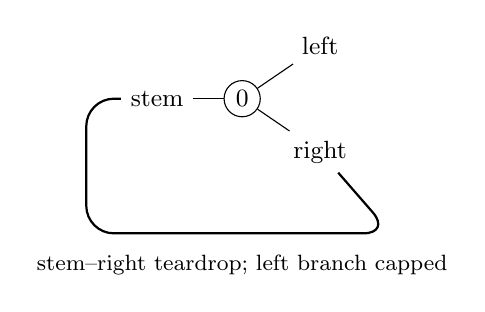
\begin{tikzpicture}[scale=0.9,every node/.style={font=\small}]
  \node[draw,circle,inner sep=2pt] (s) at (0,0) {$0$};
  \node (stem) at (-1.2,0) {stem};
  \node (l) at (1.1,0.75) {left};
  \node (r) at (1.1,-0.75) {right};
  \draw (s) -- (stem); \draw (s) -- (l); \draw (s) -- (r);
  \draw[thick,rounded corners=10pt]
    (stem) -- (-2.2,0) -- (-2.2,-1.9) -- (2.1,-1.9) -- (r);
  \node at (0,-2.35) {\footnotesize stem--right teardrop; left branch capped};
\end{tikzpicture}
\end{center}

Start the train entering the right branch (port $2$) with tongue
$\Left$.  The trailing entry pins the tongue to $\Right$ and exits the
stem; the stem's edge leads back into port $2$.  The two sampled times
already show both vectors:
\[
\begin{array}{c|c|c}
  \text{time} & \text{entering port} & \text{tongue of switch }0\\\midrule
  0 & 2 & \Left\\
  1 & 2 & \Right
\end{array}
\]
So $f(1) = 2 = 2^1$.  (Thereafter the vector stays $\Right$: the run is
live forever but mints nothing new --- a first taste of the upper bound.)

\subsection{$N = 2$: the dogbone Gray square}

\begin{construction}\label{con:dogbone}
  Join the two branches of switch $0$ to each other ($w(1)=2$), the two
  branches of switch $1$ to each other ($w(4)=5$), and the two stems to
  each other ($w(0)=3$).
\end{construction}

\begin{center}
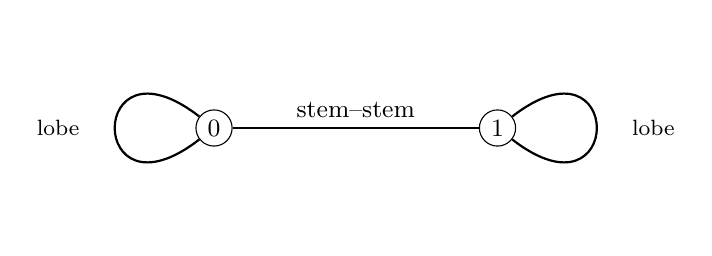
\begin{tikzpicture}[scale=0.9,every node/.style={font=\small}]
  \node[draw,circle,inner sep=2pt] (a) at (0,0) {$0$};
  \node[draw,circle,inner sep=2pt] (b) at (4,0) {$1$};
  \draw[thick] (a) -- node[above]{stem--stem} (b);
  \draw[thick] (a) .. controls (-1.8,1.4) and (-1.8,-1.4) .. (a);
  \draw[thick] (b) .. controls (5.8,1.4) and (5.8,-1.4) .. (b);
  \node at (-2.2,0) {\footnotesize lobe};
  \node at (6.2,0) {\footnotesize lobe};
\end{tikzpicture}
\end{center}

Each branch-to-branch loop is a \emph{lobe}: a train leaving the stem
comes around the lobe and re-enters through the \emph{other} branch,
trailing, which flips that switch's tongue --- lobes alternate.  Start
the train entering the stem of switch $0$ with both tongues $\Left$
(write a vector as the pair $u(0)u(1)$).  Every second step completes one
lobe pass and flips one tongue, walking the full Gray cycle of the
$2$-cube:
\[
\begin{array}{c|c|c}
  \text{time} & \text{entering port} & \text{vector}\\\midrule
  0 & 0 \text{ (stem }0\text{)} & \Left\Left\\
  2 & 3 \text{ (stem }1\text{)} & \Right\Left\\
  4 & 0 \text{ (stem }0\text{)} & \Right\Right\\
  6 & 3 \text{ (stem }1\text{)} & \Left\Right
\end{array}
\]
(The odd times enter the lobes' far branches: ports $2, 5, 1, 4$.)  All
four vectors of two switches appear, so $f(2) = 4 = 2^2$.  The next flip
returns to $\Left\Left$ at time $8$: the run cycles through the square
forever.

\section{Attainment for $N \ge 3$: the extremal family}\label{sec:family}

Now $\min(2^N, N+4) = N+4$, and one explicit family of layouts attains
it for every $N \ge 3$ (\lean{state\_law\_lower\_bound}, file
\file{StateLawLowerBound.lean}; found empirically by a Python state-count
prober, then proved symbolically in $N$).

\begin{construction}[The extremal wiring]\label{con:family}
  On switches $0,\dots,N-1$:
  \begin{itemize}
  \item switch $0$ carries a lobe (its two branches joined,
    $w(1) = 2$), and its stem is joined to the stem of switch $1$
    ($w(0) = 3$) --- together a teardrop hanging at the bottom;
  \item switches $1,\dots,N-3$ form a chain: the right branch of switch
    $k$ is joined to the stem of switch $k+1$;
  \item switches $N-2$ and $N-1$ are doubly linked: the left branch of
    $N-2$ to the stem of $N-1$, and right branch to right branch.
  \end{itemize}
  All other ports are unwired.
\end{construction}

\begin{center}
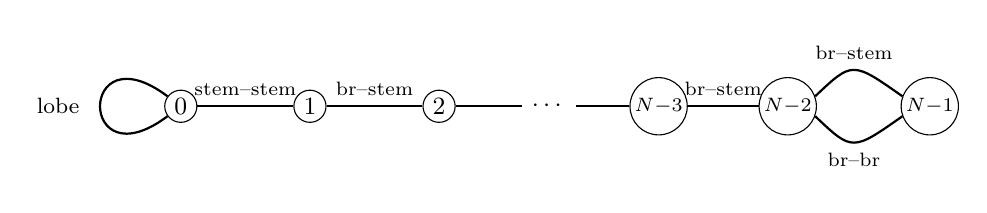
\begin{tikzpicture}[scale=0.82,every node/.style={font=\small}]
  \node[draw,circle,inner sep=1.5pt] (t) at (0,0) {$0$};
  \draw[thick] (t) .. controls (-1.6,1.2) and (-1.6,-1.2) .. (t);
  \node at (-1.9,0) {\footnotesize lobe};
  \node[draw,circle,inner sep=1.5pt] (c1) at (2,0) {$1$};
  \node[draw,circle,inner sep=1.5pt] (c2) at (4,0) {$2$};
  \node (dots) at (5.7,0) {$\cdots$};
  \node[draw,circle,inner sep=1pt] (cn3) at (7.4,0) {\scriptsize $N{-}3$};
  \node[draw,circle,inner sep=1pt] (cn2) at (9.4,0) {\scriptsize $N{-}2$};
  \node[draw,circle,inner sep=1pt] (cn1) at (11.6,0) {\scriptsize $N{-}1$};
  \draw[thick] (t) -- node[above]{\scriptsize stem--stem} (c1);
  \draw[thick] (c1) -- node[above]{\scriptsize br--stem} (c2);
  \draw[thick] (c2) -- (dots); \draw[thick] (dots) -- (cn3);
  \draw[thick] (cn3) -- node[above]{\scriptsize br--stem} (cn2);
  \draw[thick] (cn2.20) .. controls (10.4,0.7) .. node[above]{\scriptsize br--stem} (cn1.160);
  \draw[thick] (cn2.-20) .. controls (10.4,-0.7) .. node[below]{\scriptsize br--br} (cn1.200);
\end{tikzpicture}
\end{center}

\begin{theorem}[Lower bound, $N \ge 3$]\label{thm:lower}
  On the wiring of Construction~\ref{con:family}, the cold start ---
  entering the right branch of switch $N-2$ with all tongues $\Left$ ---
  is live at the $N+4$ times
  \[ 0,\ 1,\ \dots,\ N-2,\quad N,\quad 2N-1,\quad 2N,\quad 3N-1,\quad
     4N-1, \]
  and the restricted tongue vectors at those times are pairwise
  distinct.  Hence $f(N) \ge N+4$.
\end{theorem}

\begin{proof}[Proof (rendered)]
  Identify a vector with its set of $\Right$ switches.  The run has four
  phases, and the sampled vectors are:

  \begin{center}
  \begin{tabular}{ll}
    \toprule
    time & vector ($\Right$-set)\\
    \midrule
    $0,1,\dots,N-2$ &
      $\varnothing,\ \{N{-}2\},\ \{N{-}3,N{-}2\},\ \dots,\
       \{1,\dots,N{-}2\}$\\
    $N$ & $\{0,1,\dots,N{-}2\}$\\
    $2N-1$ & $\{0,\dots,N{-}1\}$\\
    $2N$ & $\{0,\dots,N{-}1\}\setminus\{N{-}2\}$\\
    $3N-1$ & $\{0,\dots,N{-}1\}\setminus\{N{-}2,0\}$\\
    $4N-1$ & $\{0,\dots,N{-}1\}\setminus\{0\}$\\
    \bottomrule
  \end{tabular}
  \end{center}

  \emph{Phase 1 (descent, times $0,\dots,N-2$).}  The cold train enters
  the right branch of $N-2$ trailing, pinning $N-2$ to $\Right$ and
  leaving by its stem, which is wired to the right branch of $N-3$; the
  trailing cascade rolls down the chain, pinning one new switch per step
  --- each sampled prefix mints a new vector.

  \emph{Phase 2 (teardrop, times $N-1,\dots$).}  From the stem of switch
  $1$ the train reaches the stem of switch $0$ facing.  Its tongue says
  $\Left$, so the train exits by the left branch into the lobe and comes
  back through the right branch, trailing: switch $0$ flips to $\Right$
  (the time-$N$ vector).  Emerging from stem $0$ it re-enters stem $1$
  facing; each chain switch's tongue now points at the branch the train
  arrived by in Phase~1, so the train retraces the chain \emph{backwards
  by pure facing moves, changing nothing} (the retrace mechanism of
  Section~\ref{ssec:cascade}), reaching the stem of switch $N-2$ at time
  $2N-3$.  Its tongue, set to $\Right$ in Phase~1, sends the train out
  the right branch, and the right--right link delivers it into the right
  branch of switch $N-1$ at time $2N-2$.

  \emph{Phase 3 (closing the far switch).}  That trailing entry sets
  $N-1$ to $\Right$: at time $2N-1$ all $N$ switches are $\Right$.  The
  train leaves by the stem of $N-1$, whose link leads into the
  \emph{left} branch of $N-2$, trailing --- so $N-2$ flips to $\Left$
  at time $2N$ (the train now heading down the chain again).

  \emph{Phase 4 (the Gray oscillation).}  From here the run oscillates
  on the two coordinates $N-2$ and $0$ only: down the chain (trailing
  entries that change nothing), around the teardrop lobe --- which
  flips switch $0$ --- back up by facing retrace, and around the double
  link --- which flips $N-2$: the tongue of $N-2$ decides whether the
  train arrives at $N-1$ through its stem or its right branch, and
  either way it returns into the other branch of $N-2$.  Concretely,
  $0$ flips to $\Left$ at time $3N-1$, $N-2$ back to $\Right$ at $4N-1$,
  $0$ back to $\Right$ at $5N-2$, and so on with period $3N-1$: the four
  corners of the square are visited in Gray order, and times $3N-1$ and
  $4N-1$ sample the two corners not yet seen.

  Distinctness is a matter of pointing at one differing coordinate for
  each pair, and the table makes the witness explicit: within Phase~1,
  coordinate $N-1-m$ separates the $m$-th prefix from the later ones;
  coordinate $0$ separates Phase~1 from time $N$; coordinate $N-1$
  separates times $\le N$ from times $\ge 2N-1$; and the four late
  vectors differ on $\{N-2, 0\}$, where they realise the four
  combinations.  (In the formal text the trajectory claims are proved by
  induction on each phase and the liveness and distinctness checks are
  explicit; the $N = 3$ base case, where the chain is empty, is checked
  by the kernel.)
\end{proof}

\section{The sharp upper bound: $f(N) \le N+4$}\label{sec:upper}

This is the mathematical core.  The formal statement
(\lean{state\_law\_N\_add\_four}) is exactly the upper-bound half of
Theorem~\ref{thm:main}; its proof occupies most of the development.
What follows is a faithful map of that argument: every definition and
numbered claim below corresponds to a formal one, and the file named in
brackets is where it lives.  Proofs here are proof \emph{sketches} ---
the intended level is ``the reader sees why it is true and what must be
checked''; the formal text is the complete verification.

Throughout, fix a wiring $w$ on switches $0,\dots,N-1$.

\subsection{Trailing cascades and the retrace lemma}\label{ssec:cascade}

The engine of everything is the asymmetry of the lazy point: trailing
passes write, facing passes read.

\begin{lemma}[Cascades are wiring-determined; \file{GeneralN.lean}]
  \label{lem:cascade}
  A trailing entry exits by the stem regardless of the tongues.  Hence a
  maximal run of consecutive trailing passes (a \emph{cascade}) --- its
  route, and the pins it writes --- depends only on the wiring and the
  entry port, not on the tongue vector.
\end{lemma}

\begin{lemma}[Retrace; \file{GeneralN.lean}]\label{lem:retrace}
  After a cascade, enter the \emph{stem} of its last switch with any
  tongue vector agreeing with the cascade's pins.  Then the walk performs
  pure facing moves that traverse the cascade backwards, touches no
  tongue, and emerges over the cascade's original entry edge.
\end{lemma}

\begin{proof}[Sketch]
  Each cascade pass pinned its switch's tongue toward the branch the
  train entered by.  Arriving later at that switch's stem, the tongue
  therefore selects exactly that branch: the train is routed back along
  the edge it came in by, facing, changing nothing.  Induction along the
  cascade.
\end{proof}

This one-switch fact --- a passage leaves the points set so that
immediately traversing it backwards is a no-op
(\lean{arrive\_back}, \file{TrackTrace.lean}) --- is why grooves,
teardrops bounce, and long paths are re-walked for free.  We say a path
is \emph{grooved} at a vector $u$ when every passage of the path is the
one $u$ selects, and call a path \emph{switch-simple} if it visits each
switch at most once.  A switch-simple path has at most $N$ passages, and
any tongue changes it makes survive to its endpoint.

\subsection{First revisit: cycles and manufactured reflectors}
\label{ssec:traces}

Follow the train from its start and record the \emph{physical trace}:
the sequence of local passages.  Because there are finitely many
switches, some switch is eventually revisited; the analysis of the
\emph{first} revisit is the fork in the whole proof
(\file{TrackTrace.lean}, \file{TrackLobe.lean},
\file{TripleSelfLinkSimpleCycleClosure.lean}).

\begin{lemma}[First-revisit dichotomy]\label{lem:dichotomy}
  Consider the first time the switch-simple initial exploration re-enters
  a switch it has already visited.  Up to the symmetric cases, one of:
  \begin{enumerate}
  \item the walk closes a \emph{simple cycle} and settles on it: after a
    switch-simple transient, the trajectory becomes periodic over a
    switch-simple cycle whose vector no longer changes; or
  \item the walk closes a \emph{lobe} (re-enters the old switch by its
    other branch) or bounces off a \emph{self-link/cap}: the layout has
    \emph{manufactured a reflector}.
  \end{enumerate}
\end{lemma}

\begin{definition}[Manufactured reflectors; \file{TrackTheta.lean}]
  \label{def:reflector}
  A \emph{manufactured reflector} on entry edge $e \to g$ consists of a
  switch-simple \emph{runway} from $g$ to a \emph{mouth}, together with
  either
  \begin{itemize}
  \item (\emph{stay reflector}) a self-linked arm at the mouth --- the cap
    reflects the train back through the branch it came by, re-pinning the
    same tongue: the local action is the identity; or
  \item (\emph{flip reflector}) a lobe at the mouth (the \emph{candy}) ---
    the far contact returns the train through the other branch, so each
    complete traversal flips exactly the mouth switch's tongue (the
    \emph{action switch}).
  \end{itemize}
  In both cases the return journey is the runway retraced backwards
  (Lemma~\ref{lem:retrace}): a complete traversal leaves every tongue
  unchanged except possibly the one action switch, and exits over the
  entry edge $e$.  The switches of runway and candy are the reflector's
  \emph{reusable support}; the action switch of a flip reflector is
  deliberately \emph{not} counted in it.
\end{definition}

The state-side consequences are the first two entries of the budget:

\begin{lemma}[Construction history; \file{FirstReflectorNovelty.lean},
  \file{SharpStateLawAssembly.lean}]\label{lem:history}
  The complete first manufacturing journey --- switch-simple exploration,
  contact, and reverse runway --- exhibits at most $N+2$ distinct
  restricted vectors: the at most $N+1$ vectors along the switch-simple
  exploration (one new tongue write per step at distinct switches,
  starting from the initial vector), plus at most one for the activated
  state.  The activation itself, however long the runway, contributes at
  most that single new vector, because the return is a retrace.
\end{lemma}

\begin{lemma}[Two-phase and four-corner laws;
  \file{ManufacturedPairNovelty.lean}, \file{TrackThetaAllTime.lean}]
  \label{lem:phases}
  A complete traversal of a manufactured reflector has exactly two tongue
  phases: the incoming vector, and that vector with the local action
  applied.  For \emph{two} opposite reflectors $A, B$ bouncing a train
  between them, every vector at every time lies in the four algebraic
  corners
  \[ u,\quad u + A,\quad u + B,\quad u + A + B, \]
  whether or not their supports intersect: if the supports avoid each
  other this is the composed two-phase law, and if one action lands on
  the other's grooved support the \emph{theta} analysis
  (\file{TrackTheta*.lean}) shows the disturbed groove is either repaired
  in one trailing pass or captured into the old mouth, giving pointwise
  covers by at most three or four vectors.  No path length ever enters:
  the covers are blind to how long the runways are.
\end{lemma}

The dogbone of Section~\ref{sec:small} is the equality case of
Lemma~\ref{lem:phases}, and the cap-versus-lobe distinction is exactly
the sticky/alternating dichotomy visible in the toy.

\subsection{The coordinate budget}\label{ssec:budget}

All counting is funnelled through one frame
(\file{TrackFiniteAlternation.lean}).  Call a live step
\emph{productive} if it changes the restricted vector; its \emph{writer}
is the switch it enters.  Then a run's distinct vectors are at most
\[ 1 \;+\; \#\{\text{first productive writes}\} \;+\;
   \#\{\text{repeated-writer novelties}\}, \]
where the first term is the initial vector, the second is at most $N$
--- one per switch --- and a \emph{repeated-writer novelty} is a
productive event of an already-productive switch whose resulting vector
is globally new.  The whole difficulty of the theorem is that repeated
writers may in principle keep minting new vectors; the reflector
machinery exists to cap them by a constant.  The refined bookkeeping
never charges the crude $N$: it charges the switch-simple
\emph{exploration} (at most $N$ coordinates, Lemma~\ref{lem:history}),
and every later count is charged \emph{into the same $N$ ambient switch
coordinates} --- reusable support here, productive first writers of a
continuation there --- plus explicitly named constant corners.  Two
overlapping histories are never paid twice: when a second manufactured
exploration follows a first, the union of the two construction histories,
with their shared boundary vector erased, still fits the frame
(\file{TwoHistoryUnionCharge.lean},
\file{TwoJourneyTailCountSharp.lean}).

\subsection{The probe tree after one reflector}\label{ssec:probe}

Assume now the run's \emph{incoming edge is known}: it entered its start
over a wired edge (the general start is lifted in
Section~\ref{ssec:boundary}).  The first-revisit dichotomy
(Lemma~\ref{lem:dichotomy}) and a second probe of $N+1$ raw steps after
the first reflector generate a finite tree of outcomes, each closed by
its own count (files \file{PartialSecondRunSharp.lean},
\file{PartialSecondRunNAddFour.lean},
\file{OneReflectorContinuation.lean},
\file{FirstCycleCountSharp.lean}):

\begin{center}
\begin{tabular}{lll}
  \toprule
  outcome & count & mechanism\\
  \midrule
  death before any revisit & $\le N+1$ & switch-simple prefix\\
  settles on a simple cycle & $\le N+2$ &
    transient $+$ repeat and settled vectors\\
  reflector, then dead probe & $\le N+2$ &
    dead runs cannot damage the support\\
  reflector, then stable cycle & $\le N+3$ &
    joint charge of support and writers\\
  reflector, then changed contact & $\le N+4$ & Lemma~\ref{lem:contact}\\
  two opposite protected reflectors & $\le N+4$ & Lemma~\ref{lem:pair}\\
  \bottomrule
\end{tabular}
\end{center}

The two $N+4$ leaves are the genuine frontier
(\file{KnownEdgeNAddFourFrontier.lean}); everything else in the tree is
$N+3$ or less.

\begin{lemma}[Changed contact; \file{ChangedContactNAddFour.lean},
  \file{KnownEdgeNAddFourChangedClosed.lean}]\label{lem:contact}
  Suppose after the first flip reflector the run makes a first
  support-changing contact.  The general changed-support count pays a
  compressed lead of $N+3$ plus two fresh Gray corners; but the
  reflector's facing action switch is deliberately absent from its
  reusable support, so unless the strict pre-contact approach
  productively first-writes that very switch, the action switch is a
  reserved ambient coordinate, the lead compresses to $N+2$, and the
  branch closes at $N+4$.  In the remaining action-written case the local
  forward tail has only one fresh corner (a runway alternative is killed
  by the retrace contradiction), which again yields $N+3+1 = N+4$.
\end{lemma}

\begin{lemma}[Protected pair; \file{ProtectedPairNAddFour.lean},
  \file{PreReturnProtectedRoute.lean}, \file{CompleteRepairFour.lean}]
  \label{lem:pair}
  Suppose the second probe manufactures a second reflector opposite the
  first, with each action avoiding the other's support (the
  \emph{protected pair}).  The two construction histories overlap: either
  the first reflector's omitted facing mouth is the second construction's
  first productive writer --- then its post-write vector duplicates the
  first reflector's pre-return vector, and erasing the duplicate gives an
  $N+2$ construction cover, to which the protected repair tail adds at
  most two novelties (Lemma~\ref{lem:phases}) --- or the overlap analysis
  degrades gracefully through the explicitly enumerated remaining cases
  (repair leads have two phases,
  \file{RepairLeadTwoPhase.lean}; facing-forward and backward-contact
  futures cost a constant, \file{FacingForwardNovelty.lean},
  \file{TrackEarlyRepairConstant.lean},
  \file{StateLawTwoCandidate.lean}).  Every case totals at most $N+4$.
\end{lemma}

Packaging the closed tree gives the keystone:

\begin{theorem}[Known incoming edge;
  \lean{knownIncomingEdgeNAddFour},
  \file{KnownEdgeNAddFourComplete.lean}]\label{thm:knownedge}
  If the start is entered over a wired edge, every duplicate-free list of
  live sample times with pairwise-distinct restricted vectors has length
  at most $N+4$.
\end{theorem}

\subsection{Arbitrary starts and the productive boundary}
\label{ssec:boundary}

A general start need not arrive over an edge --- the train may simply be
placed at a port.  Consider its very first passage
(\file{StateLawNAddFourTop.lean}).  If that passage is \emph{quiet}
(changes no restricted tongue --- a facing entry, or a trailing entry
that re-pins), then from time $1$ on the run has a known incoming edge,
and the time-zero vector equals the time-one vector, so
Theorem~\ref{thm:knownedge} absorbs it.  The only danger is a
\emph{productive first passage}: the train is dropped into a branch of
some switch $k_0$ and its very first move flips $k_0$, so the original
vector $u$ exists only at time zero, and the shifted run --- which starts
at $u$ with $k_0$ flipped, over a known edge --- might use its full
$N+4$ budget on top of it.

\begin{proposition}[Productive boundary;
  \lean{ProductiveInitialBoundaryNAddFour},
  \file{StateLawNAddFourSharp.lean}]\label{prop:boundary}
  The time-zero vector of a productive first passage is never an extra
  state: the shifted run together with the original vector still fits in
  $N+4$.
\end{proposition}

\begin{proof}[Sketch]
  Suppose adjoining $u$ exceeds the budget.  Then the shifted run is
  \emph{saturated}: it attains all $N+4$ of its vectors, every one of its
  live vectors is among the sampled ones, and $u$ itself never occurs on
  it (\file{BoundaryNAddFourSaturation.lean}).  Saturation is a very
  rigid situation, and the geometry of the first journey narrows it to
  two \emph{savings}, each worth the one missing unit:
  \begin{itemize}
  \item \emph{Absent saving.}  The boundary switch $k_0$ never occurs in
    the first manufactured exploration.  Then $k_0$ is a genuinely unused
    coordinate of the first support; if it is also absent from the second
    construction's productive first writers, adjoining $u$ is paid by
    this reserved coordinate outright
    (\file{BoundaryAbsentSecondWriter.lean},
    \file{BoundaryAbsentProtectedPair.lean}).
  \item \emph{Occurrence saving.}  The initially written switch is met
    again, unchanged, inside the first journey.  A canonical such
    occurrence forces, via the entry-edge symmetry, an empty runway and a
    literal self-link (\file{BoundaryCanonicalGeometry.lean}); a
    noncanonical one supplies a \emph{second} repeated vector in the
    first journey, and erasing both repetitions makes room to insert $u$
    into the history at no cost (\file{BoundaryDoubleDuplicate.lean},
    \file{BoundaryResidualNovelty.lean},
    \file{BoundaryOccurrenceDamageElimination.lean}).
  \end{itemize}
  What remains after the savings are spent are the support-damage
  outcomes, and both expose \emph{the same} sharp changed contact of the
  first reflector --- the damaged stable cycle through its lead, the
  damaged opposite reflector through its exploration.  Under the absent
  saving, the shifted run begins at the boundary switch's own stem, so
  switch-simplicity makes $k_0$ automatically reserved along the strict
  approach and closes every such contact at $N+3$
  (\file{BoundaryChangedContactSaving.lean},
  \file{BoundaryApproachActionElimination.lean}); under the occurrence
  saving, the occurrence replacement closes the same contact
  (\file{BoundaryResidualSharpening.lean}).  Together with the outright
  eliminations of the short outcomes (a dead second probe and a preserved
  second cycle are too small to saturate,
  \file{ProductiveBoundaryNAddFourComplete.lean}), every saturated
  configuration is contradictory, which proves the proposition.
\end{proof}

\begin{theorem}[Sharp upper bound; \lean{state\_law\_N\_add\_four}]
  \label{thm:upper}
  For every wiring on switches $0,\dots,N-1$, every start, and every
  duplicate-free list of live sample times with pairwise-distinct
  restricted vectors, the list has length at most $N+4$.
\end{theorem}

\begin{proof}
  Split the samples at time zero.  A quiet first passage reduces to
  Theorem~\ref{thm:knownedge} directly; a productive first passage is
  Proposition~\ref{prop:boundary}.  (\file{StateLawNAddFourTop.lean}
  performs this bookkeeping exactly.)
\end{proof}

\section{Assembly}\label{sec:assembly}

\begin{proof}[Proof of Theorem~\ref{thm:main}]
  \emph{Upper bound:} a duplicate-free sample list is bounded by $2^N$
  (Proposition~\ref{prop:ceiling}) and by $N+4$
  (Theorem~\ref{thm:upper}), hence by their minimum.
  \emph{Attainment:} for $N = 0$ the empty layout, for $N = 1$ the
  teardrop, for $N = 2$ the dogbone (Section~\ref{sec:small}), each
  attaining $2^N = \min(2^N, N+4)$; for $N \ge 3$ the extremal family
  (Theorem~\ref{thm:lower}) attains $N+4$, which is the minimum by
  Lemma~\ref{lem:minside}.
\end{proof}

\section{About the formalisation}\label{sec:formal}

The development lives in \file{theory/lean} of the repository and builds
with Lean~4 (toolchain 4.32.2) and no external library:
\begin{center}
  \texttt{lake build}
\end{center}
compiles all $70$ files and ends by printing the axiom audit of the
single theorem:
\begin{center}
  \lean{GeneralN.state\_law} depends on axioms:
  \lean{[propext, Classical.choice, Quot.sound]}.
\end{center}
Points worth recording:

\begin{itemize}
\item \emph{One theorem.}  \lean{state\_law} in \file{StateLaw.lean} is
  the only headline statement; every other declaration is reachable
  support --- the tree is mechanically verified to be exactly the
  theorem's dependency closure.
\item \emph{Trusted base.}  The three axioms are Lean's standard ones.
  There is no \lean{sorry} and no \lean{native\_decide}: the finite
  witness runs of Section~\ref{sec:small} and the $N = 3$ base of
  Theorem~\ref{thm:lower} are evaluated by the proof kernel
  (\lean{decide}).  No definition uses choice to produce data (the
  development contains no \lean{noncomputable} declaration); classical
  reasoning appears only as excluded middle inside proofs.
\item \emph{Symbolic in $N$.}  The upper bound and the $N \ge 4$ lower
  bound contain no finite-instance argument: all inductions are
  structural in the trace or in $N$.
\item \emph{Provenance.}  The extremal family was found by an empirical
  state-count prober; the geometry of the physical pieces never enters
  the proofs, which is itself a (machine-checked) modelling statement:
  plain track only transports the train between ports.
\end{itemize}

\begin{center}
\begin{tabular}{ll}
  \toprule
  entry point & contents\\
  \midrule
  \file{StateLaw.lean} & the theorem and its statement language\\
  \file{StateLawSmallN.lean} & $2^N$ ceiling; empty/teardrop/dogbone\\
  \file{StateLawLowerBound.lean} & the extremal family, $N \ge 3$\\
  \file{StateLawNAddFourTop.lean} & arbitrary-start bookkeeping\\
  \file{KnownEdgeNAddFourComplete.lean} & the known-edge $N+4$ theorem\\
  \file{TrackTrace.lean}, \file{TrackTheta.lean} & traces, reflectors,
    theta engine\\
  \file{StateLawAxiomAudit.lean} & the axiom audit\\
  \bottomrule
\end{tabular}
\end{center}

\end{document}
